\documentclass{article}
\usepackage[T1]{fontenc}
\usepackage[utf8]{inputenc}
\usepackage[portuguese]{babel}

\usepackage{hyphenat}

\title{A preencher}
\author{Lucas Emanuel Resck Domingues}
\date{Novembro 2019}

\usepackage{natbib}
\usepackage{graphicx}
\usepackage{amsmath}
\usepackage{amssymb}
\usepackage{subcaption}

\begin{document}

    \maketitle

    \begin{abstract}
        A preencher
    \end{abstract}
    
    \newpage

    \tableofcontents

    \newpage

    \section{Introdução}

        Redes neurais são uma subárea da inteligência artificial que busca aprender relações e padrões de forma semelhante a um cérebro biológico.
        Atualmente, a utilização de redes neurais já está estabelecida, e toda grande empresa ou instituição que lida com tecnologia já faz seu uso.
        Porém, assim como nosso cérebro, ainda não temos um grau de entendimento suficiente do seu funcionamento.

        Uma rede complexa é um grafo.
        Geralmente ela é caracterizada pelo fato de não ser possível explicar \textit{features} emergentes apenas pela soma de suas partes.
        Por exemplo, é muito difícil entender como uma doença se propaga olhando apenas para como um indivíduo pega e transmite uma doença.
        
        Dessa maneira, redes neurais podem ser interpretadas como redes complexas.
        Na verdade, a teoria de redes complexas tem se mostrado útil para seu entendimento \cite{galhardo2006redes}.
        Poucos trabalhos, porém, têm sido realizados nesse sentido.

        O objetivo deste trabalho é introduzir algumas arquiteturas de redes neurais (rede neural tradicional \textit{feedfoward} e rede de crença profunda)
        e apresentar e analisar alguns resultados do estudo de redes de crença profunda do ponto de vista de redes complexas, por \cite{testolin2018deep}.
        Serão apresentadas medidas de topologia de grafos (como grau e "força" \ médios) em uma rede de crença profunda antes e depois do seu treinamento.
        Além disso, serão exploradas relações entre funcionais dos neurônios e a estrutura da rede (será que a função que um neurônio desempenha afeta a relação entre o grau e a força médios, por exemplo?).

        Este é um trabalho avaliado para a disciplina Tópicos de Matemática Aplicada, com relação à área de Redes Complexas, com aulas ministradas pelo professor Moacyr Alvim Horta.

    \section{Redes neurais \textit{feedforward}}
        \label{feedforward}

        Esta seção introduz uma configuração de redes neurais chamada \textit{feedforward}, como exemplifica a Figura \ref{fig1}, apresentada em \cite{nielsen2015neural}.

        \begin{figure}[h!]
            \centering
            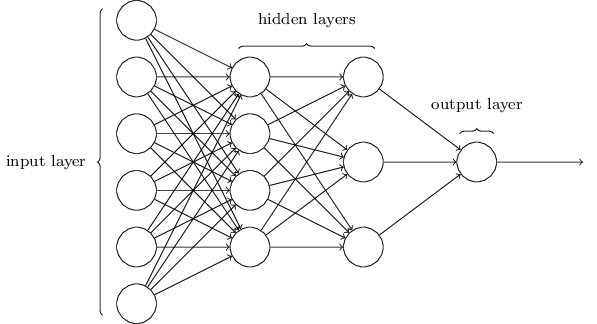
\includegraphics[scale=0.5]{Images/Feedforward neural network.png}
            \caption{Exemplo de rede neural \textit{feedforward}.}
            \label{fig1}
        \end{figure}        

        \subsection{Neurônios sigmóide}

            A unidade fundamental de uma rede neural é o neurônio, em analogia ao cérebro presente nos animais.
            Sejam $x_1, \cdots, x_n$ valores numéricos de entrada pertencentes a $[0, 1]$.
            Um neurônio é uma função que toma esses valores como entrada e produz uma saída, como exemplifica a Figura \ref{fig2}, também apresentada por \cite{nielsen2015neural}.

            \begin{figure}[h!]
                \centering
                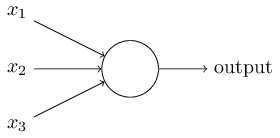
\includegraphics[scale=0.5]{Images/Sigmoid neuron.png}
                \caption{Exemplo de neurônio.}
                \label{fig2}
            \end{figure}
            
            Porém, esses neurônios não são uma função qualquer. Na verdade, podem ser descritos como:

            \begin{equation}
                \begin{split}
                    \textrm{output} &= \sigma(\mathbf{w} \cdot \mathbf{x} + \mathbf{b}) \\
                                    &= \dfrac{1}{1 + e^{-(\mathbf{w} \cdot \mathbf{x} + \mathbf{b})}}
                \end{split}
            \end{equation}

            $\sigma$ é a função sigmóide, daí o nome "neurônio sigmóide".

            $\mathbf{w}$ é um vetor de pesos, podendo ser interpretados como os pesos das arestas que ligam $x_i$ e o neurônio.
            Seu objetivo é "levar em consideração" \ todas as entradas, porém ponderando essas configurações.
            Veremos mais tarde, neste trabalho, que o objetivo da rede neural é "aprender" \ (também) quais os valores de $\mathbf{w}$.

            $\mathbf{x}$ é o vetor da entrada.
            
            $\mathbf{b}$ é um vetor de viéses.
            Quando os neurônios não usavam funções sigmóide, a saída era $0$ ou $1$.
            O objetivo do viés, então, era deslocar o parâmetro em que o neurônio seria "ativado" \ ou não.

            Observe que a saída do neurônio é uma função não linear de uma combinação linear das entradas.
            A combinação linear permite que ajustemos os pesos para a saída que quisermos, ou seja, "pequenas alterações na entrada produzem pequenas alterações na saída".
            A ideia é que não geramos saltos ou grandes variações quando alteramos apenas um pouco o parâmetro de entrada.
            
            O fato da função ser não linear é o que dá a complexidade da função quando muitos neurônios são reunidos.
            Veremos que, ao reunirmos vários neurônios para formar uma rede neural, teremos uma função não linear muito complexa.

        \subsection{Arquitetura}

            A arquitetura de uma rede neural tradicional se dá criando partições de um grafo.
            Observe novamente a Figura \ref{fig1}.
            A cada partição do grafo, chamaremos camada (\textit{layer}).
            Duas camadas "adjacentes" \ são totalmente conectadas, com todas as arestas orientadas no mesmo sentido (que, por convenção, será da esquerda para a direita).

            A primeira camada é chamada camada de entrada (\textit{input layer}).
            Tecnicamente, esta não é uma camada de verdade, mas apenas uma representação da entrada de valores, tal que os neurônios para os quais as arestas dessa camada apontam apenas recebem esses valores.
            
            A última camada é a de saída (\textit{output}).
            As camadas restantes são chamadas escondidas (\textit{hidden layers}), apenas por analogia.

            Vamos considerar a matriz $W_k$ sendo aquela com os pesos da camada $k$.
            Então o elemento $w_{ji}$ (linha $j$, coluna $i$) representa o peso da aresta que liga o nó $j$ da camada $k$ ao nó $i$ da camada $k + 1$.
            Além disso, $b_k$ representa os viéses de cada neurônio da camada $k$.
            
            Dessa forma, um vetor $\mathbf{x}$ na camada $k$ tem como resultado na camada $k + 1$ o vetor $\sigma (W_{ji} \mathbf{x} + \mathbf{b_k})$.
            Observe que a função $\sigma(\mathbf{x})$ aplicada ao vetor $\mathbf{x}$ representa a aplicação da função $\sigma$ a todos os elementos de $\mathbf{x}$.

            Sejam $W$ a matriz tridimensional de $W_k$ e $b$ a matriz de vetores $\mathbf{b_k}$.

        \subsection{Aprendizado com o método do gradiente}
        
            Suponha que queiramos uma rede neural para diferenciar gatos e cachorros.
            Então construímos de forma que tenha dois neurônios na camada de saída.
            Queremos que, ao alimentarmos a rede com a imagem (vetorizada) e um cachorro, ela resulte em um vetor $(1, 0)$.
            Quando alimentada por uma imagem de um gato, $(0, 1)$.
            Buscamos um banco de dados de cachorros e gatos. Seja $\mathbf{y}$ a função que identifica cachorros e gatos:

            \begin{equation}
                \mathbf{y}(\mathbf{x}) =    \begin{cases}
                                                (1, 0), & \textrm{se } \mathbf{x} \textrm{ representa um cachorro}, \\
                                                (0, 1), & \textrm{se } \mathbf{x} \textrm{ representa um gato}
                                            \end{cases}
            \end{equation}

            Se $a$ é a função que representa nossa rede neural e temos $n$ imagens, definimos a função \textbf{custo}:
            
            \begin{equation}
                C(W, b) = \dfrac{1}{2n} \sum_{\mathbf{x}} ||\mathbf{y}(\mathbf{x}) - a(\mathbf{x}, W, b)||^2
            \end{equation}

            Nosso objetivo, nesse sentido, é calcular $W$ e $b$ tal que a função custo seja mínima.
            O método utilizado para isso é o do gradiente (\textit{gradient descent}), que atualiza os vetores $\mathbf{w_k}$ e $\mathbf{b_l}$ da seguinte forma:

            \begin{equation}
                \begin{split}
                    \mathbf{w_k} &\rightarrow \mathbf{w_k'} = \mathbf{w_k} - \eta \dfrac{\partial C}{\partial \mathbf{w_k}} \\
                    \mathbf{b_l} &\rightarrow \mathbf{b_l'} = \mathbf{b_l} - \eta \dfrac{\partial C}{\partial \mathbf{b_l}}
                \end{split}
            \end{equation}

            Porém, como $C = (\sum_{\mathbf{x}} C_{\mathbf{x}}) / n$, então
            
            \begin{equation}
                \dfrac{\partial C}{\partial \mathbf{w_k}} = \dfrac{1}{n} \sum_{\mathbf{x}} \dfrac{\partial C_{\mathbf{x}}}{\partial \mathbf{w_k}}
            \end{equation}
            
            O cálculo para todo $\mathbf{x}$ pode ser custoso, então introduzimos o método do gradiente estocástico (\textit{stochastic gradient descent}), de modo que escolhemos uma amostra aleatória $X_1, \cdots, X_m$ do nosso banco de dados (um "mini-batch") e calculamos:

            \begin{equation}
                \begin{split}
                    \mathbf{w_k} &\rightarrow \mathbf{w_k'} = \mathbf{w_k} - \dfrac{\eta}{m} \sum_j \dfrac{\partial C_{X_j}}{\partial \mathbf{w_k}} \\
                    \mathbf{b_l} &\rightarrow \mathbf{b_l'} = \mathbf{b_l} - \dfrac{\eta}{m} \sum_j \dfrac{\partial C_{X_j}}{\partial \mathbf{b_l}}
                \end{split}
            \end{equation}

            As derivadas, por sua vez, são calculadas utilizando \textit{backpropagation}.

    \section{Rede de crença profunda}
        \label{belief}

        Em \cite{testolin2018deep}, foi utilizada outro tipo de arquitetura de redes neurais, a chamada rede de crença profunda (\textit{deep belief network}).
        A topologia é muito semelhante, mas ela é diferente no modo como ocorre o aprendizado.

        \subsection{Máquina de Boltzmann restrita}

            Uma máquina de Boltzmann restrita é um grafo bipartite em que as duas partições são totalmente conectadas por arestas não orientadas, como mostra a Figura \ref{fig3}, apresentada em \cite{testolin2018deep}.

            \begin{figure}[h!]
                \centering
                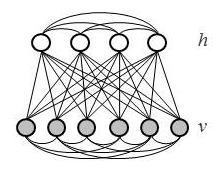
\includegraphics[scale=0.5]{Images/Restricted Boltzmann machine.png}
                \caption{Máquina de Boltzmann restrita.}
                \label{fig3}
            \end{figure}

            A camada $v$ é chamada camada visível, pois é aquela que recebe o vetor de entrada.
            A camada $h$ é a camada escondida. Como na rede \textit{feedforward}, as arestas têm pesos, porém não há viéses.

            Nesta configuração de redes, os neurônios são ativados ($1$) ou não ($0$), diferentemente da configuração anterior, em que os neurônios pudiam assumir valores entre $[0, 1]$.
            Seja $W$ a matriz de pesos dessa rede, e $w_{ji}$ um elemento.
            Dado um vetor $\mathbf{v}$ na camada visível, a ativação $\mathbf{h}$ dos neurônios na camada é dada por:

            \begin{equation}
                h_i =   \begin{cases}
                            1, \ \textrm{com probabilidade } \dfrac{1}{1 + e^{-\sum_j w_{ji} v_j}},\\
                            0, \ \textrm{caso contrário}.
                        \end{cases}
                \label{hi}
            \end{equation}

            O aprendizado dessa rede acontece em duas fases, que, em \cite{testolin2018deep}, são chamadas de fases \textbf{positiva} e \textbf{negativa}.
            Na fase positiva, fornecemos um vetor $\mathbf{v}$ à camada visível, e o vetor $\mathbf{h}$ é calculado de acordo com a equação \ref{hi}.

            Na fase negativa, ao invés de colocarmos um vetor na camada de entrada, a rede automaticamente gera um vetor nessa camada, iniciando aleatoriamente um vetor na camada escondida.

            Dessa forma, são atualizados os pesos da rede de acordo com

            \begin{equation}
                \Delta w_{ij} = \epsilon(\mathbb{E}_{\textrm{dados}}(v_i h_j) - \mathbb{E}_{\textrm{modelo}}(v_i h_j))
            \end{equation}

            em que $\mathbb{E}_{\textrm{dist}}$ é o valor esperado sob a distribuição especificada: distribuição empírica (fase positiva) e a distribuição do modelo (fase negativa).
            $\epsilon$ é uma contante chamada taxa de aprendizado.
            
            Esse modelo é chamado de máquina de Boltzmann restrita pois há um grafo bipartite, em contraste com a máquina de Boltzmann convencional, em que a rede é totalmente conectada.

        \subsection{Rede de crença profunda}

            Uma rede de crença profunda é uma composição de máquinas de Boltzmann restritas. Observe a Figura \ref{fig4}, apresentada em \cite{testolin2018deep}.

            \begin{figure}[h!]
                \centering
                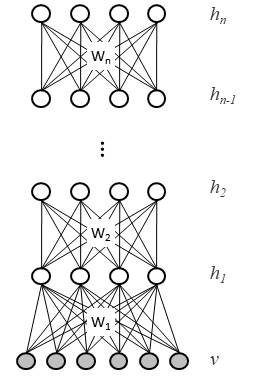
\includegraphics[scale=0.5]{Images/Deep belief network.png}
                \caption{Rede de crença profunda.}
                \label{fig4}
            \end{figure}

            Nessa rede, há uma camada visível e $n$ camadas escondidas.
            Para treinar essa rede, treina-se a primeira máquina de Boltzmann restrita ($v$ e $h_1$).
            Após isso, utiliza-se as atividades dos neurônios em $h_1$ para treinar a máquina de Boltzmann composta por $h_1$ e $h_2$.
            E assim por diante.

            A ideia nesse tipo de rede é que, à medida que atividades escondidas vão sendo utilizadas como entrada, a rede vai construindo representações mais abstratas dos dados (\cite{testolin2018deep}), assim como em uma rede neural tradicional.

    \section{Análise de redes neurais a partir de ciência de redes}
        \label{analysis}

        Em \cite{testolin2018deep}, é explorada uma rede de crença profunda utilizando ferramentas de ciência de redes e redes complexas.
        A ideia é que, quando se inicia uma rede de crença profunda com pesos aleatórios (neste trabalho, dados por uma distribução normal com média zero), padrões emergem.
        O foco, portanto, será apontar alguns avanços obtidos por \cite{testolin2018deep} a partir de uma rede treinada com imagens de dígitos manuscritos (base de dados MNIST), utilizando três máquinas de Boltzmann restritas (MBR).
        Se $W_i$ é a matriz de adjacência de cada MBR, então esta é a matriz de toda a rede de crença:

        \begin{equation}
            W = \begin{bmatrix}
                    0 & W_1 & 0 & 0 \\
                    W_1^T & 0 & W_2 & 0 \\
                    0 & W_2^T & 0 & W_3 \\
                    0 & 0 & W_3^T & 0
                \end{bmatrix}
        \end{equation}

        Pontos que são abordados:
        
        \begin{itemize}
            \item Distribuição dos graus, "forças" \ (a ser definido) e pesos em cada camada;
            \item Grau médio, "força", coeficiente de variação e vizinhos próximos médios das subredes formadas por nós com propriedades funcionais similares (veja Seção \ref{field}).
        \end{itemize}

        Para o cálculo da distribuição dos graus não ser trivial (rede totalmente conectada), foi estabelecido um limiar (\textit{threshold}) $\theta$, de modo a zerar arestas com peso menor do que $\theta$.

        \subsection{Campos receptivo neuronais}
            \label{field}

            Um campo receptivo é basicamente como um neurônio "vê" \ o vetor de entrada.
            Suponha um neurônio na primeira camada escondida.
            O modo como ele "vê" \ a entrada depende basicamente dos pesos das arestas que ligam os nós da camada de entrada e ele próprio.
            Se todos os pesos forem $0$, então o neurônio não vê nada.
            Essa característica de cada nó é importante, pois a partir dela é possível perceber as \textit{features} que são importantes em cada nó e camada.

            O campo receptivo dos nós de outras camadas é uma combinação linear dos campos dos nós das camadas anteriores.

            \begin{figure}[h!]
                \centering
                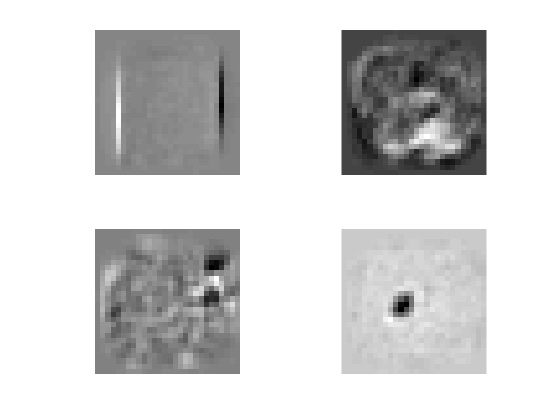
\includegraphics[scale=0.2]{Images/Receptive fields.png}
                \caption{Exemplo de campos receptivos (apresentado em \cite{testolin2018deep}).}
                \label{fig5}
            \end{figure}

            Os autores decidiram dividir os nós do grafo em grupos para algumas das análises, e realizam o agrupamento baseado nos campos receptivos, utilizando algumas técnicas pertinentes.

        \subsection{Resultados}

            A Figura \ref{fig6} (de \cite{testolin2018deep}) mostra os resultados da distribuição dos pesos antes e depois do aprendizado.

            \begin{figure}[h!]
                \begin{subfigure}{0.5\textwidth}
                    \centering
                    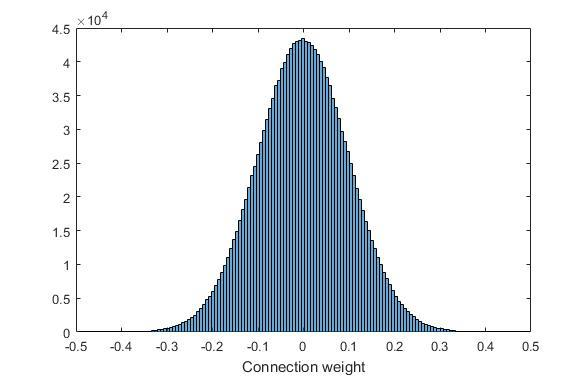
\includegraphics[scale=.3]{Images/Weights distribution.png}
                    \caption{Toda a rede antes do treinamento.}
                \end{subfigure}
                \begin{subfigure}{0.5\textwidth}
                    \centering
                    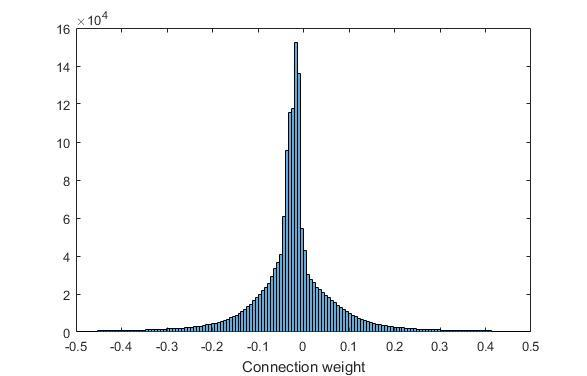
\includegraphics[scale=0.3]{Images/Weights distribution (2).png}
                    \caption{Toda a rede depois do treinamento.}
                \end{subfigure}
                \begin{subfigure}{0.5\textwidth}
                    \centering
                    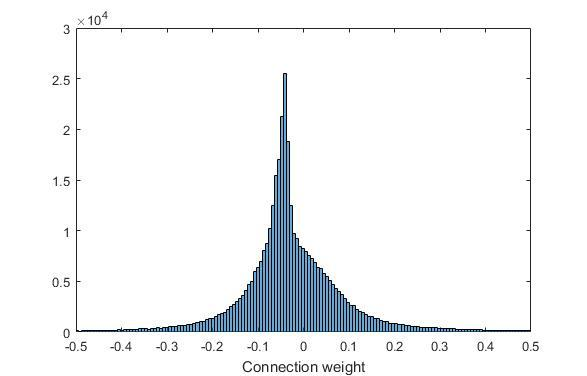
\includegraphics[scale=0.3]{Images/Weights distribution (3).png}
                    \caption{$v - h1$ depois do treinamento.}
                \end{subfigure}
                \begin{subfigure}{0.5\textwidth}
                    \centering
                    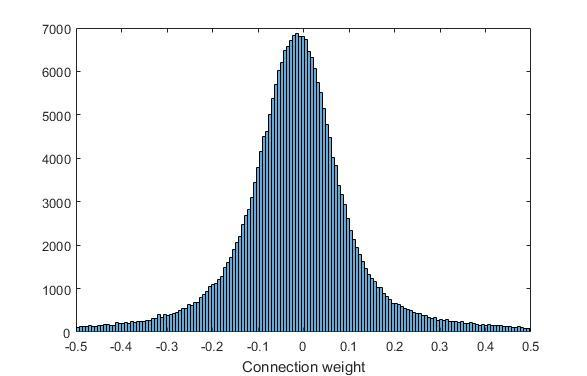
\includegraphics[scale=0.3]{Images/Weights distribution (4).png}
                    \caption{$h1 - h2$ depois do treinamento.}
                \end{subfigure}
                \begin{center}
                    \begin{subfigure}{0.5\textwidth}
                        \centering
                        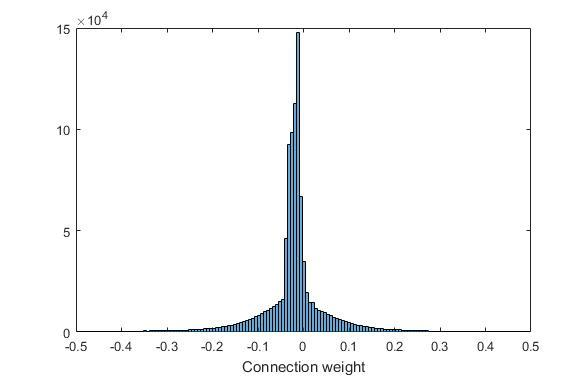
\includegraphics[scale=0.3]{Images/Weights distribution (5).png}
                        \caption{$h2 - h3$ depois do treinamento.}
                    \end{subfigure}
                \end{center}
                \caption{Distribuição dos pesos da rede.}
                \label{fig6}
            \end{figure}

            \begin{itemize}
                \item Houve um deslocamento para a esquerda da distribuição dos pesos da rede como um todo;
                \item A distribuição não é mais gaussiana (principalmente por $v - h1$ e $h2 - h3$);
                \item $h1 - h2$ ainda é quase normal, mas com maior variância e caudas mais longas.
            \end{itemize}

            A força de um nó $i$ pode ser definida como $s_i = \sum_j w_{ij}$. Alguns resultados:

            \begin{itemize}
                \item No início, a distribuição é gaussiana, por consequência da distribuição dos pesos ser gaussiana;
                \item Em geral, após o treinamento, as forças foram negativas;
                \item Existem longas caudas positivas;
                \item As forças dos nós em $v - h1$ são todas negativas.
            \end{itemize}

            Em relação aos campos receptores, os nós do início da rede (primeira camada) possuem campos que representam estruturas localizadas simples, como pequenas manchas,
            enquanto aqueles mais profundos representam \textit{features} mais complexas, como detecção de arestas.

            Agora vamos analisar alguns resultados que relacionam características topológicas (estrutura da rede) e características funcionais (campos receptores).
            Consideramos subredes $G_i$ formadas por nós que pertencem ao mesmo grupo de campos receptores.
            Foram estudadas as seguintes características topológicas:

            \begin{itemize}
                \item Grau médio de nós: $\overline{k_i} = \sum_{j \in G_i} k_j / |G_i|$, em que $k_j$ é o grau do nó $j$ e $|G_i|$ é o número de nós na subrede $G_i$;
                \item Grau positivo médio de nós: $\overline{k_i^+} = \sum_{j \in G_i, k_j \ge 0} k_j / |G_i|$;
                \item Grau negativo médio de nós: $\overline{k_i^-} = \sum_{j \in G_i, k_j \le 0} k_j / |G_i|$;
                \item Grau médio de vizinhos próximos: $\overline{k_{nn_i}} = \sum_{i \in G_i} \sum_{j \in nn(i)} k_j / G$, em que $nn(i)$ são os vizinhos próximos de $i$ e $G$ é o número de subgrafos (19, no nosso caso);
                \item Força média dos nós: $\overline{s}_i = \sum_{j \in G_i} s_j / G$, em que $s_j$ é a força do nó $j$.
            \end{itemize}

            A Figura \ref{fig6} (apresentada em \cite{testolin2018deep}) mostra alguns resultados comparando as medidas acima para os subgrafos e camadas.

            \begin{figure}[h!]
                \centering
                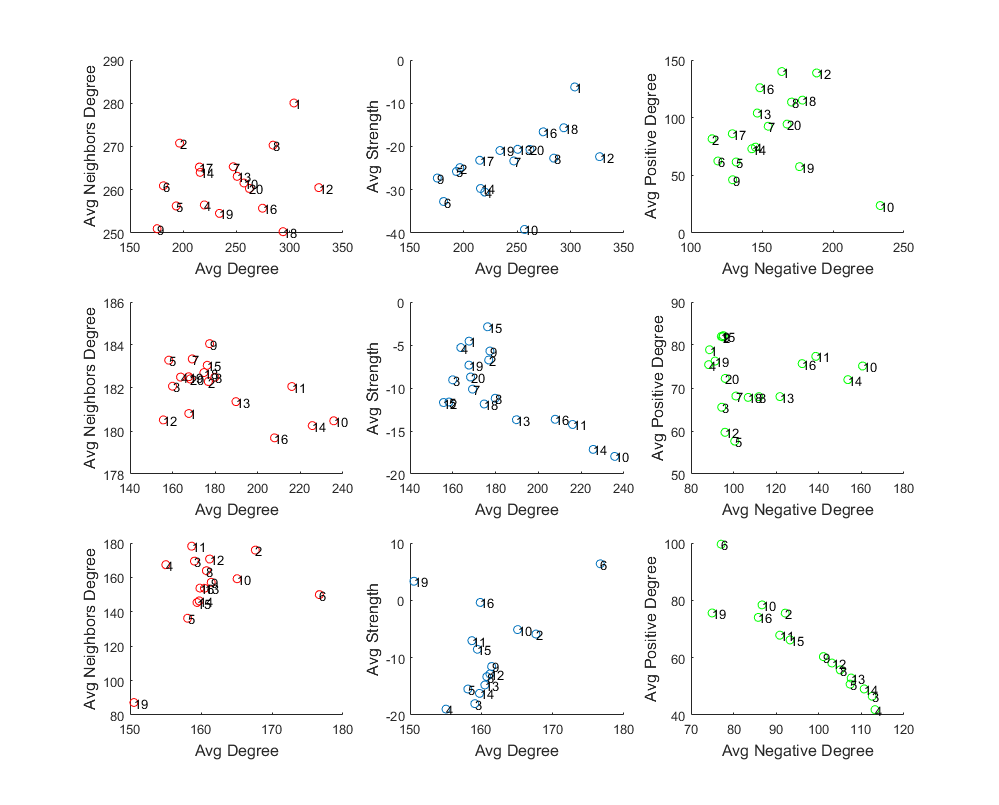
\includegraphics[scale=0.35]{Images/Structure vs function.png}
                \caption{Resultados do estudo de características topológicas e funcionais.
                Cada linha representa uma camada, cada coluna representa uma comparação.
                Cada ponto é uma medida topológica de um subgrafo.}
                \label{fig6}
            \end{figure}

            Alguns resultados, portanto:

            \begin{itemize}
                \item Vemos que não há clara correlação entre grau médio de nós e o grau médio de vizinhos próximos (coluna da esquerda).
                \item Há uma correlação nas três camadas entre força média dos nós e grau médio dos nós (coluna do meio).
                \item Há em partes correlação entre grau médio positivo dos nós e grau médio negativo: isso ocorre nas primeira e terceira camadas (coluna da direita).
            \end{itemize}

    \section{Considerações finais}

        Os objetivos principais deste trabalho foram estudar algumas arquiteturas de redes neurais e investigar uma rede neural da perspectiva de ciência de redes e redes complexas.

        As redes neurais \textit{feedforward} tradicionais são algumas das pioneiras, das mais simples e das mais compreensíveis.
        Bibliotecas, \textit{softwares} e métodos de utilizar esse tipo de rede não faltam, mostrando por que é pertinente estudar essa arquitetura.
        \cite{nielsen2015neural} foi um ótimo guia introdutório para isso.
        
        A necessidade do estudo de redes de crença profunda surgiu para que fosse possível compreender os resultados em \cite{testolin2018deep}.
        Realmente, pouco trabalho existe no que diz respeito à interseção entre redes neurais e redes complexas, e \cite{testolin2018deep} foi uma das exceções.

        Os resultados apresentados para grau médio dos nós levou em consideração um limiar $\theta$, como evidenciado na Seção \ref{analysis}.
        Se não fosse o caso, teríamos que um grafo tetapartite totalmente conectado, pela própria arquitetura da rede.

        A partir dos resultados, pudemos observar que houve uma tendência de deslocamento dos pesos em direção a valores negativos.
        Em \cite{testolin2018deep}, os autores pontuam que o contraste entre o fundo preto e os dígitos brancos pode ter induzido fortes anti-correlações entre os neurônios.
        Vários neurônios obtiveram pesos negativos, inibindo, portanto, a atividade de vários neurônios conectados.
        Seu campo receptivo, por sua vez, tende a se especializar em \textit{features} muito específicas das imagens, ativando sob estímulos muito particulares, estando anti-correlacionada com os pixels restantes da imagem.

        Ou seja, podemos pensar que muitos neurônios se especializaram em \textit{features} específicas, descartando o restante da imagem (com pesos negativos), de modo que a distribuição dos pesos da rede se moveu na direção negativa.

        Os autores comentam sobre a não trivialidade de se caracterizar módulos funcionais em redes neurais.
        A solução encontrada foi aproximar o funcional de um neurônio pelo seu campo receptivo, ou seja, aquilo que o neurônio "vê" \ e o leva a tomar uma decisão de se ativar ou não.
        Os campos receptivos foram agrupados, de modo a termos subredes de nós com campos receptivos parecidos.

        Comenta-se atualmente sobre a dificuldade de interpretabilidade de como uma rede neural toma uma decisão, como se fosse uma "caixa preta".
        Dessa forma, trabalhos que tentam "desvendá-la" \ são muito bem-vindos. 

    \bibliographystyle{plain}
    \bibliography{references}
\end{document}
